 \subsection{Поиск грамсета по конечным буквосочетаниям (алгоритм GramGuess) и по псевдоокончанию (алгоритм GramPseudoGuess)}

Для оценки алгоритмов GramGuess и GramPseudoGuess были использованы \num{73 395} пар <<слово - грамсет>> для собственно карельского наречия и  \num{452 790} пар <<слово - грамсет>> для вепсского языка. 

Для каждого слова определялся список грамсетов, упорядоченный по числу подобных словоформ, имеющих тот же грамсет.

Для оценки качества результатов поисковых алгоритмов была предложена следующая функция $\text{eval}(g^u)$:
\begin{equation}\label{eq:metric-eval-gram}
\text{eval} \left( 
    \begin{array}{@{}l@{\thinspace}l}
       g^u, \\
       \text{Counter} & \left[ g^k \right] \rightarrow c^k,\\
                      & \forall k = \overline{1,m} \\
    \end{array}
    \right)     = 
        \begin{cases}
            \multicolumn{2}{l}{\bluecomment{Массив Counter[\,] 
                  не содержит правильного грамсета $g^u$.}}\\
            0, & g^u \ne g^k, \forall k = \overline{1,m},\\[3mm]
            \multicolumn{2}{l}{\bluecomment{\specialcell{Первые несколько грамсетов в массиве могут иметь \\ 
                  одинаковую максимальную частоту $c^1$, \\
                  один из этих грамсетов совпадает с $g^u$.}}}\\
            1, & g^u \in \{ \left[ g^1, \ldots, g^j \right] : 
                               c^1=\ldots=c^j, j \leq m \},\\[4mm]
            \multicolumn{2}{l}{\frac{c^k}{ \sum_{k=1}^{m}c^k }, \; 
                \exists \, k : g^k = g^u, \;
                            c^k < c^1
                }
        \end{cases}
\end{equation}

Эта функция~(\ref{eq:metric-eval-gram}) оценивает результаты алгоритмов GramGuess и GramPseudoGuess при условии, что нам известен правильный грамсет $g^u$.

\begin{table}
	\caption{Оценка результатов поиска грамсета для вепсского и карельского языков по алгоритмам GramGuess и GramPseudoGuess.}	
	\label{tab:Gram:quantity}

% The space between the text and the left/right border of its
\setlength{\tabcolsep}{8pt}

\begin{tabular}{ c c c c c} \toprule
     & \multicolumn{2}{c}{GramGuess}& \multicolumn{2}{c}{GramPseudoGuess}\\ \cmidrule(r){2-5}
%     &       GramGuess & & GramPseudoGuess & \\ \cmidrule(r){2-5}     
                                                
 Оценка & вепсский & карельский & вепсский & карельский\\ \midrule
0 & 2.53 & 5.72 & 7.9 & 9.23\\
0.1 & 0.53 & 0.83 & 1.04 & 1.57\\
0.2 & 0.71 & 1.16 & 1.24 & 1.37\\
0.3 & 0.64 & 0.89 & 2.68 & 1.36\\
0.4 & 0.2 &	0.56 & 0.14 & 0.68\\
0.5 & 0.11 & 0.09 & 0.83 & 0.43\\
1 &	\textbf{95.29} & \textbf{90.74} & \textbf{86.17} & \textbf{85.36}\\
\bottomrule
\end{tabular}
\end{table}

В таблице 4 видно, что алгоритм GramGuess показал себя лучше, чем GramPseudoGuess, а именно: 

\begin{labeling}{eval-formula}
% Среди найденных частей речи отсутствует правильная у 4.7% вепсских слов и у 9% карельских слов (x=0 на рис.4).
\item [карельский] 
%90.7\% versus 85.4\% for Karelian and 95.3\% versus 85.4\% for Veps.
90.7\% карельским словам был присвоен правильный грамсет по алгоритму GramGuess против 85.4\% по алгоритму GramPseudoGuess;
\hfill \break

\item [вепсский] 
95.3\% вепсским словам был присвоен правильный грамсет по алгоритму GramGuess против 85.4\% по алгоритму GramPseudoGuess.
\end{labeling}

Возможно причина в том,  что конечные буквосочетания длиннее псевдоокончаний и дают больше информации. 
К тому же алгоритм GramPseudoGuess не подходит для частей речи без флективных форм.


\subsection{Анализ ошибок алгоритмов поиска по аналогии}

% TODO нарисовать картинку для третьего алгоритма, 
% где для неизвестного слова u
% поочерёдно подбираются существующие слова из словаря 
% со всё укорачивающимся псевдоокончанием...
Для анализа ошибок были взяты результаты работы алгоритма POSGuess и визуализированы с помощью программы Graphviz.
% Доля и число ошибок в определении части речи, визуализация с помощью инструмента Graphviz
%
%
% Построены графы ошибок перехода для определения части речи 
% алгоритмом POSGuess для вепсского (рис. 7а)
% fig:pos-error-graph-vep
% и собственно карельского наречия карельского языка (рис. 7б).
% fig:pos-error-graph-krl
%
Были построены графы ошибок перехода для определения части речи алгоритмом POSGuess для вепсского
(рис.~\ref{fig:pos-error-graph-vep}) и собственно карельского наречия карельского языка (рис.~\ref{fig:pos-error-graph-krl}).

Объясним, как этот граф построен.
% Рассмотрим на правом рисунке (рис. 7б) толстую зелёную вертикальную стрелку с метками 21.6%, 1424, 3.9%, соединяющую прилагательные и существительные.
Например, толстая серая вертикальная стрелка соединяет прилагательные и существительные (рис.~\ref{fig:pos-error-graph-krl}), и эта стрелка имеет метки 21.6\%, 1424 and 3.9\%. 
Это означает, что алгоритм POSGuess ошибочно определил 1424 карельских прилагательных как существительные. 
Это составило 21.6\% от всех карельских прилагательных и 3.9\% от существительных.
Это можно объяснить тем, что
одна и та же лемма (в вепсском и карельском) может выступать в роли существительно и прилагательного. 
То есть в обоих языках есть одинаковые леммы для существительных и прилагательных.
Они и склоняются одинаково.

Эксперимент показал, что в нашей выборке таких лемм для собственно 
карельского языка существенно больше, чем для вепсского языка 
(21.6\% против 9.8\% на рис.~\ref{fig:pos-error-graph}). 
Хотя в абсолютных числах вепсский превышает карельский, а именно: 
6061 против 1424 ошибок такого рода. Это объясняется большим размером вепсского словаря в ВепКар.

\begin{figure}
\centering
\begin{subfigure}{.5\textwidth}
  \centering
  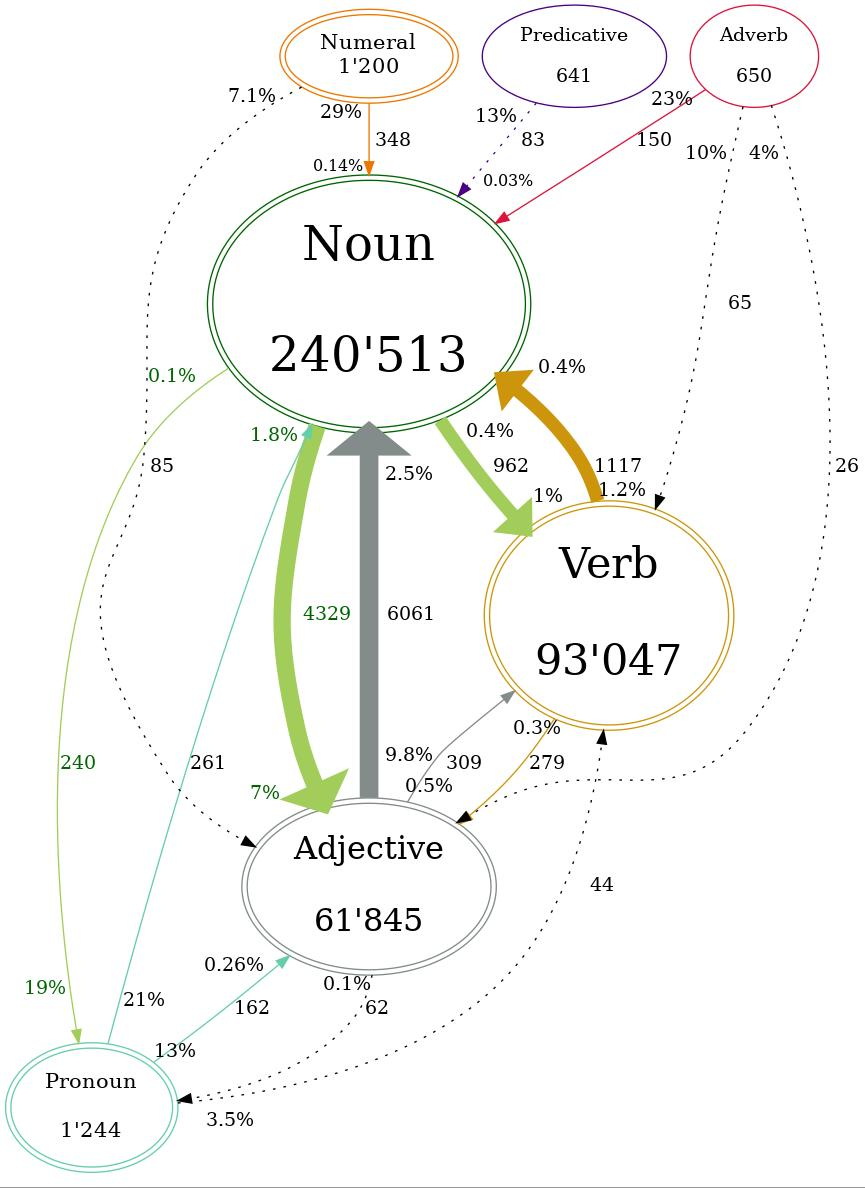
\includegraphics[width=0.95\textwidth]{experiments/247_veps_only_max0_pos-1_0.jpg}
  \caption{вепсский язык}
  \label{fig:pos-error-graph-vep}
\end{subfigure}%
\begin{subfigure}{.5\textwidth}
  \centering
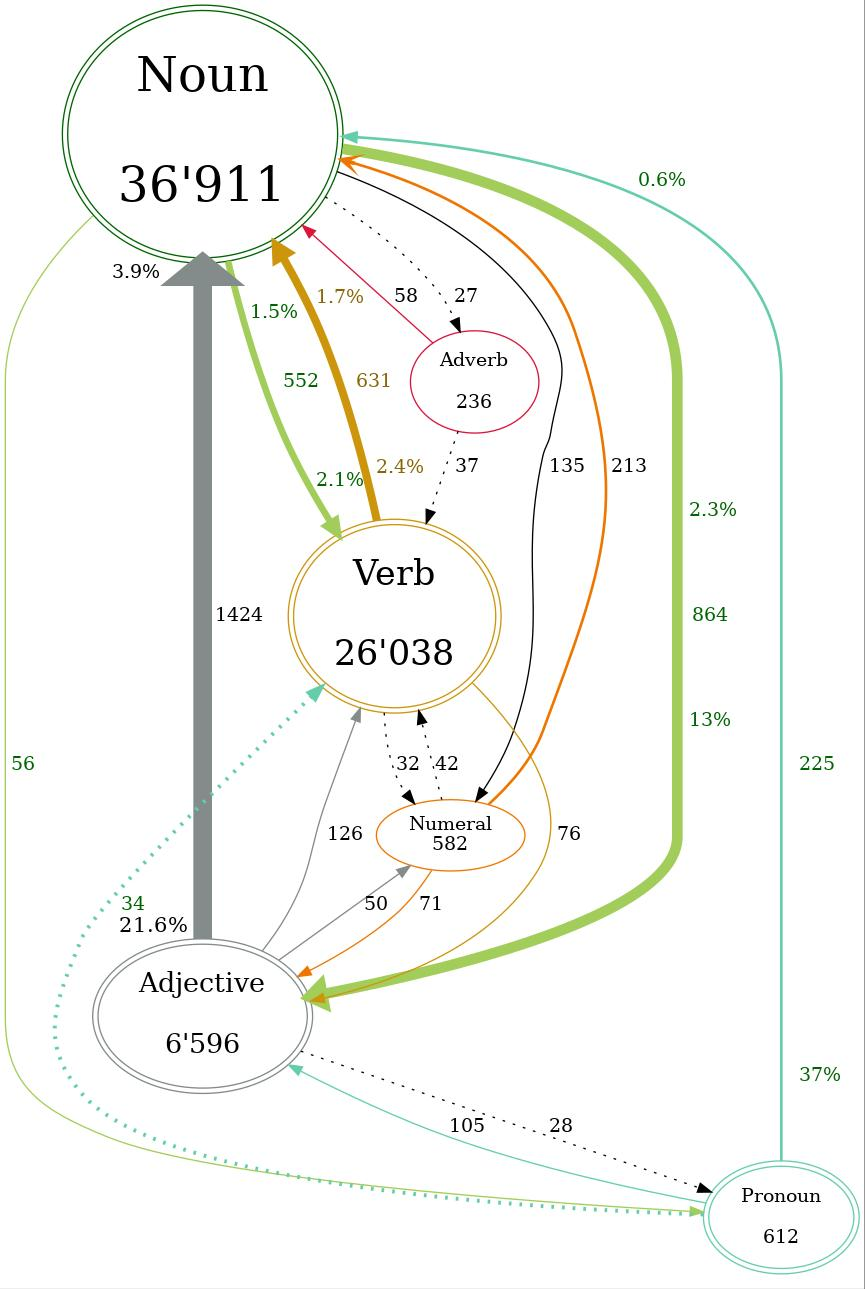
\includegraphics[width=1.0\textwidth]{experiments/456_pos-4_20_number-krl.jpg}  \caption{собственно карельское наречие карельского языка}
  \label{fig:pos-error-graph-krl}
\end{subfigure}
\caption{Граф перехода ошибок поиска части речи, который отражает результаты алгоритма POSGuess. }
\label{fig:pos-error-graph}
\end{figure}
